\documentclass[a4paper,12pt]{article}
\title{Assignment 1}
\author{ZHU Cai\\
Student No.: 09902510R\\
Department of Applied mathematics}
\usepackage{graphics}
\usepackage{Sweave}
\begin{document}
\maketitle
This assignment is programed and calculated using R-2.10.1.\\

\noindent\textbf{Question 1}\\

\noindent First, we calculate the means of stock T and stock B,
\begin{Schunk}
\begin{Sinput}
> returnrate_a <- c(0.19, 0.08, -0.12, -0.03, 0.15)
> returnrate_b <- c(0.08, 0.03, -0.09, 0.02, 0.04)
> m_a <- mean(returnrate_a)
> m_b <- mean(returnrate_b)
> round(m_a, 4)
\end{Sinput}
\begin{Soutput}
[1] 0.054
\end{Soutput}
\begin{Sinput}
> round(m_b, 4)
\end{Sinput}
\begin{Soutput}
[1] 0.016
\end{Soutput}
\end{Schunk}
from the results, we can see that Stock T is most desirable. Next, we calculate the standard deviations,
\begin{Schunk}
\begin{Sinput}
> sd_a <- sd(returnrate_a)
> sd_b <- sd(returnrate_b)
> round(sd_a, 4)
\end{Sinput}
\begin{Soutput}
[1] 0.1282
\end{Soutput}
\begin{Sinput}
> round(sd_b, 4)
\end{Sinput}
\begin{Soutput}
[1] 0.0635
\end{Soutput}
\end{Schunk}
from the results, we can see that Stock B is most desirable.\\
\noindent Finally, we calculate the Shape Radio, from definition, we know Shape Radio can be calculated as follows:\\
\begin{equation}
\centering
Shape\ Radio = \frac{R-R_f}{\sigma_R}
\end{equation}
where $R_f$ is the risk free rate.
\begin{Schunk}
\begin{Sinput}
> rf <- 0.02
> R_a <- (m_a - rf)/sd_a
> R_b <- (m_b - rf)/sd_b
> round(R_a, 4)
\end{Sinput}
\begin{Soutput}
[1] 0.2653
\end{Soutput}
\begin{Sinput}
> round(R_b, 4)
\end{Sinput}
\begin{Soutput}
[1] -0.063
\end{Soutput}
\end{Schunk}
from the results, we can see that Stock T is most desirable.\\

\noindent\textbf{Question 2}\\

\noindent (a) For 6-month apartment lease\\
\noindent if the couple stay in apartment A, they should pay (present value) :\\
\begin{Schunk}
\begin{Sinput}
> renta <- 1000
> df <- 1/(1 + 0.01)
> power <- seq(0:5)
> pva <- renta * sum(df^power)
> round(pva, 0)
\end{Sinput}
\begin{Soutput}
[1] 5795
\end{Soutput}
\end{Schunk}
\noindent if the couple stay in apartment B, they should pay (present value) :\\
\begin{Schunk}
\begin{Sinput}
> rentb <- 900
> df <- 1/(1 + 0.01)
> power <- seq(0:5)
> pvb <- rentb * sum(df^power) + 1000
> round(pvb, 0)
\end{Sinput}
\begin{Soutput}
[1] 6216
\end{Soutput}
\end{Schunk}
from the result, we can see the couple should stay in apartment A.\\

\noindent (b) For 12-month apartment lease\\
\noindent if the couple stay in apartment A, they should pay (present value) :\\
\begin{Schunk}
\begin{Sinput}
> renta <- 1000
> df <- 1/(1 + 0.01)
> power <- seq(0:11)
> pva <- renta * sum(df^power)
> round(pva, 0)
\end{Sinput}
\begin{Soutput}
[1] 11255
\end{Soutput}
\end{Schunk}
\noindent if the couple stay in apartment B, they should pay (present value) :\\
\begin{Schunk}
\begin{Sinput}
> rentb <- 900
> df <- 1/(1 + 0.01)
> power <- seq(0:11)
> pvb <- rentb * sum(df^power) + 1000
> round(pvb, 0)
\end{Sinput}
\begin{Soutput}
[1] 11130
\end{Soutput}
\end{Schunk}
from the result, we can see the couple should stay in apartment B.\\

\noindent\textbf{Question 3}\\

\noindent To find the IRR is to find the root of a  polynomial, in this question, we use the bisection method.
\begin{Schunk}
\begin{Sinput}
> x0 <- -110
> x <- 35
> y0 <- -150
> y <- 40
> power <- seq(1:5)
> fn1 <- function(r1) {
+     df1 <- 1/(1 + r1)
+     pv1 <- x * sum(df1^power) + x0
+     return(pv1)
+ }
> fn2 <- function(r2) {
+     df2 <- 1/(1 + r2)
+     pv2 <- y * sum(df2^power) + y0
+     return(pv2)
+ }
\end{Sinput}
\end{Schunk}
in order to use the bisection method, we should find an inicial interval which contains the root,from
the figures, we know that the root should be in ${0.05, 0.30}$.
\begin{figure}
\centering
\scalebox{1}[0.5]{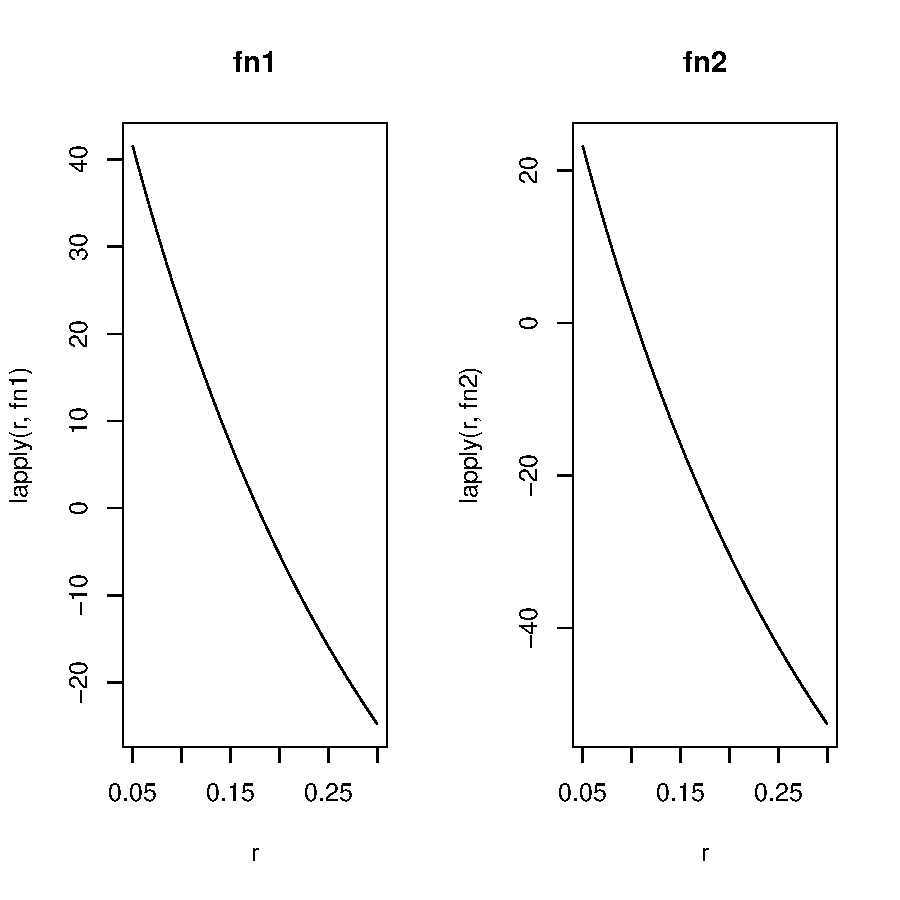
\includegraphics{assign1-010}}
\end{figure}
\begin{Schunk}
\begin{Sinput}
> setwd("C:/Documents and Settings/zc/Desktop/course-IS")
> source("bisection.R")
> IRR1 <- bisection(fn1, x.l = 0.05, x.r = 0.3)
\end{Sinput}
\begin{Soutput}
at iteration 1 the root lies between 0.175 and 0.3
at iteration 2 the root lies between 0.175 and 0.2375
at iteration 3 the root lies between 0.175 and 0.20625
at iteration 4 the root lies between 0.175 and 0.190625
at iteration 5 the root lies between 0.175 and 0.1828125
at iteration 6 the root lies between 0.175 and 0.1789062
at iteration 7 the root lies between 0.1769531 and 0.1789062
at iteration 8 the root lies between 0.1769531 and 0.1779297
at iteration 9 the root lies between 0.1774414 and 0.1779297
at iteration 10 the root lies between 0.1776855 and 0.1779297
at iteration 11 the root lies between 0.1776855 and 0.1778076
at iteration 12 the root lies between 0.1777466 and 0.1778076
at iteration 13 the root lies between 0.1777771 and 0.1778076
at iteration 14 the root lies between 0.1777924 and 0.1778076
at iteration 15 the root lies between 0.1777924 and 0.1778
at iteration 16 the root lies between 0.1777924 and 0.1777962
at iteration 17 the root lies between 0.1777943 and 0.1777962
at iteration 18 the root lies between 0.1777943 and 0.1777952
at iteration 19 the root lies between 0.1777943 and 0.1777947
at iteration 20 the root lies between 0.1777945 and 0.1777947
at iteration 21 the root lies between 0.1777945 and 0.1777946
at iteration 22 the root lies between 0.1777946 and 0.1777946
at iteration 23 the root lies between 0.1777946 and 0.1777946
at iteration 24 the root lies between 0.1777946 and 0.1777946
at iteration 25 the root lies between 0.1777946 and 0.1777946
at iteration 26 the root lies between 0.1777946 and 0.1777946
at iteration 27 the root lies between 0.1777946 and 0.1777946
at iteration 28 the root lies between 0.1777946 and 0.1777946
\end{Soutput}
\begin{Sinput}
> IRR2 <- bisection(fn2, x.l = 0.05, x.r = 0.3)
\end{Sinput}
\begin{Soutput}
at iteration 1 the root lies between 0.05 and 0.175
at iteration 2 the root lies between 0.05 and 0.1125
at iteration 3 the root lies between 0.08125 and 0.1125
at iteration 4 the root lies between 0.096875 and 0.1125
at iteration 5 the root lies between 0.096875 and 0.1046875
at iteration 6 the root lies between 0.1007812 and 0.1046875
at iteration 7 the root lies between 0.1027344 and 0.1046875
at iteration 8 the root lies between 0.1037109 and 0.1046875
at iteration 9 the root lies between 0.1041992 and 0.1046875
at iteration 10 the root lies between 0.1041992 and 0.1044434
at iteration 11 the root lies between 0.1041992 and 0.1043213
at iteration 12 the root lies between 0.1041992 and 0.1042603
at iteration 13 the root lies between 0.1042297 and 0.1042603
at iteration 14 the root lies between 0.104245 and 0.1042603
at iteration 15 the root lies between 0.104245 and 0.1042526
at iteration 16 the root lies between 0.104245 and 0.1042488
at iteration 17 the root lies between 0.1042469 and 0.1042488
at iteration 18 the root lies between 0.1042479 and 0.1042488
at iteration 19 the root lies between 0.1042483 and 0.1042488
at iteration 20 the root lies between 0.1042483 and 0.1042486
at iteration 21 the root lies between 0.1042483 and 0.1042485
at iteration 22 the root lies between 0.1042484 and 0.1042485
at iteration 23 the root lies between 0.1042484 and 0.1042485
at iteration 24 the root lies between 0.1042484 and 0.1042485
at iteration 25 the root lies between 0.1042484 and 0.1042485
at iteration 26 the root lies between 0.1042484 and 0.1042484
at iteration 27 the root lies between 0.1042484 and 0.1042484
at iteration 28 the root lies between 0.1042484 and 0.1042484
\end{Soutput}
\begin{Sinput}
> IRR1
\end{Sinput}
\begin{Soutput}
[1] 0.1777946
\end{Soutput}
\begin{Sinput}
> IRR2
\end{Sinput}
\begin{Soutput}
[1] 0.1042484
\end{Soutput}
\end{Schunk}
to calculate NPV, we discount the cash flow to the inicial time point
\begin{Schunk}
\begin{Sinput}
> r <- 0.05
> NPV1 <- fn1(0.05)
> NPV2 <- fn2(0.05)
> round(NPV1, 0)
\end{Sinput}
\begin{Soutput}
[1] 42
\end{Soutput}
\begin{Sinput}
> round(NPV2, 0)
\end{Sinput}
\begin{Soutput}
[1] 23
\end{Soutput}
\end{Schunk}
\noindent\textbf{Present value criterion:}\\
\noindent The higher the present value, the more desirable the alternative, so we choose 1;\\
\noindent\textbf{Internal rate of return criterion:}\\
\noindent The higher the internal rate of return, the more desirable the alternative, so we choose 1;\\
thus, the IRR and NPV yield same recommendations. \\

\noindent\textbf{Question 4}\\
\noindent$CFS(-2X_0, X_d + X_s)$ \\
\noindent$X_d = 1.2X_0\ ;\ \ X_s = RX_0;$\\
\noindent$R_{total} = (1.2 + R)X_0/2X_0 = (1.2 + R)/2$\\


\noindent\textbf{Question 5}\\

\noindent From the definition, the mean rate of return of the portfolio is
\begin{equation}
\centering
E(r) = E(\sum\limits_{i=1}^{n}\omega_ir_i) = \sum\limits_{i=1}^{n}\omega_iE(r_i) = \alpha\overline{r}_A + (1-\alpha)\overline{r}_B
\end{equation}
And the standard deviation is
\begin{equation}
\centering
std(r) = \sqrt{\sum\limits_{i,j=1}^{n}\omega_i\omega_j\sigma_{ij}} = \sqrt{\alpha^2\sigma_A + (1-\alpha)^2\sigma_B +
2\alpha(1-\alpha)\sigma_{AB}}
\end{equation}
\begin{Schunk}
\begin{Sinput}
> sigA <- 0.15
> sigB <- 0.05
> ro <- 0.2
> fn <- function(a) {
+     fn0 <- a^2 * 0.15^2 + (1 - a)^2 * 0.05^2 + 2 * a * (1 - a) *
+         0.05 * 0.15 * 0.2
+     fn1 <- 0.3 * a - 2 * (1 - a) * 0.05 + 2 * 0.2 * 0.15 * 0.05 *
+         (1 - 2 * a)
+     fn2 <- 0.3 + 0.1 - 2 * 0.2 * 0.15 * 0.05 * 2
+     return(c(-1 * fn0, -1 * fn1, -1 * fn2))
+ }
> source("C:/Program Files/R/R-2.10.1/work/newton.R")
> result <- newton(fn, 0.3)
> result
\end{Sinput}
\begin{Soutput}
[1] 0.2461929
\end{Soutput}
\begin{Sinput}
> std <- sqrt(-1 * fn(result)[1])
> std
\end{Sinput}
\begin{Soutput}
[1] 0.05780186
\end{Soutput}
\end{Schunk}
from the calculation, we know that the desirable $\alpha$ is 0.25, and the minimum standard deviation is 5.8\%. From the definition of $E(r)$, we know the expected return of this portfolio is 2.75\%.
\end{document}
